%% Submissions for peer-review must enable line-numbering 
%% using the lineno option in the \documentclass command.
%%
%% Preprints and camera-ready submissions do not need 
%% line numbers, and should have this option removed.
%%
%% Please note that the line numbering option requires
%% version 1.1 or newer of the wlpeerj.cls file, and
%% the corresponding author info requires v1.2

\documentclass[fleqn,10pt,lineno]{wlpeerj} % for journal submissions
% \documentclass[fleqn,10pt]{wlpeerj} % for preprint submissions

\title{Invasive lionfish present region-wide variation of allometric growth in
the Western Atlantic}

\author[1]{Juan Carlos Villaseñor-Derbez}
\affil[1]{Bren School of Environmental Sciences and Management, University of
California Santa Barbara, Santa Barbara, California, U.S.}
\corrauthor[1]{Juan Carlos Villaseñor-Derbez}{jvillasenor@bren.ucsb.edu}

% \keywords{Keyword1, Keyword2, Keyword3}

\begin{abstract}
Lionfish (\emph{Pterois volitans/miles}) are an invasive species in the
North-Western Atlantic and the Caribbean. In order to better manage the
invasion, inform lionfish removal programs, and estimate biomass
available for harvest, we must be able to accurately estimate their
total biomass, frequently from length observations. This work compares
length-weight relationships of the invasive lionfish through the
invasion with the addition of parameters for the Central Mexican
Caribbean. A review of 15 length-weight relationships reported in 10
peer-reviewed studies shows that lionfish exhibit spatial variation in
weight-at-length. The reviewed parameters indicate that, for the same
length, lionfish in the Caribbean have lower body mass than in the
Atlantic or Gulf of Mexico. This highlights the importance of using
site-specific parameters to estimate biomass from length observations.
This study also reports a new pair of length-weight parameters
(\(a = 3.2056\times 10^{-6}; b = 3.235\)) for organisms sampled in the
Central Mexican Caribbean. Findings from this work can aid managers and
decision makers to better select length-weight parameters when these are
not available for their region of interest.
\end{abstract}

\begin{document}

\flushbottom
\maketitle
\thispagestyle{empty}

\section{Introduction}\label{introduction}

At least 84\% of the marine eco-regions have reported the presence of an
invasive species \citep{molnar_2008}, which represent a major threat to
local biodiversity and the economic activities that depend on it
\citep{bax_2003}. Invasive species may threaten native species through
predation, competition, or indirect habitat effects
\citep{davis_2003, gurevitch_2004}. By 2005, the economic cost of
invasive species to the United States was estimated at USD\$120 billion
per year\citep{pimentel_2005}.

Lionfish (\emph{Pterois volitans/miles} complex) are an invasive species
in the Western Atlantic and the Caribbean, likely introduced through
liberation of aquarium-kept organisms \citep{betancurr_2011}. They are
the first marine vertebrates to establish in North Atlantic
\citep{schofield_2009,schofield_2010} and Caribbean coasts
\citep{sabidoitza_2016}. Lionfish have been widely reported in coral
reefs \citep{aguilarperera_2010}, but also in other habitats such as
estuaries \citep{jud_2011}, mangroves \citep{barbour_2010}, areas with
hard-bottoms \citep{muoz_2011}, and mesophotic reefs
\citep{andradibrown_2017}. Due to their threat to local biodiversity,
the speed of their spread, and difficulty of management, their presence
in these waters has been labeled as a major marine invasion
\citep{hixon_2016}.

A significant amount of research has been done to describe lionfish
feeding ecology in North Carolina \citep{muoz_2011}, the Bahamas
\citep{morris_2009,cote_2013}, Northern Gulf of Mexico
\citep{dahl_2014}, Mexican Caribbean
\citep{valdezmoreno_2012,villaseorderbez_2014}, Belize
\citep{hackerott_2017}, and Costa Rica \citep{sandel_2015}. Their
feeding behavior and high consumption rates can reduce recruitment
\citep{albins_2008} and population sizes \citep{green_2012} of native
reef-fish species, and further the endangerment of critically endangered
reef fish \citep{rocha_2015}. (However, see \citet{hackerott_2017} for a
case where there was no evidence that lionfish affected the density,
richness, or community composition of prey fishes). Major efforts have
been made to understand the possible impacts of the invasion by keeping
track of its range through time \citep{schofield_2009,schofield_2010}
and predicting invasion ranges under future climates
\citep{grieve_2016}. By combining information from these disciplines,
researchers have been able to predict the trophic impacts of lionfish
\citep{ariasgonzalez_2011}, which can then be translated into
ecosystem-level and economic impacts.

Seeking to reduce lionfish densities, governments and non-profit
organizations have promoted removal programs and incentivized its
consumption \citep{chin_2016}. In some cases, these have shown to
significantly reduce --but not quite eliminate-- lionfish abundances at
local scales \citep{sandel_2015,chin_2016,deleon_2013}. The rapid
recovery rates exhibited by lionfish \citep{barbour_2011} and the
persistent populations in mesophotic coral ecosystems
\citep{andradibrown_2017} --which can contribute with recruitment to
shallow-water populations-- make of complete eradication through fishing
effort an unlikely solution. However, further incentivizing its
consumption might create a demand big enough to promote and sustain a
stable fishery \citep{chin_2016}, which can reduce local abundances and
control the invasion while providing alternative livelihoods.

The feasibility of lionfish removal programs has been extensively
evaluated through field
observations\citep{usseglio_2017,sandel_2015,chin_2016,deleon_2013} and
empirical modeling \citep{barbour_2011,morris_2011,johnston_2015}. The
latter approeach models changes in biomass in response to changes in
mortality (\emph{i.e.} culling). In this case, biomass represents the
sum of all fish's individual weight. The individual weight of an
organism (Total Weight; TW) can be estimated from its Total Length (TL)
using the allometric growth equation (\(TW = aTL^b\)). Parameters \(a\)
and \(b\) for this equation exist for North Carolina
\citep{barbour_2011}, Northern \citep{fogg_2013,dahl_2014} and Southern
Gulf of Mexico \citep{aguilarperera_2016}, the Southern Mexican
Caribbean \citep{sabidoitza_2016}, Bahamas \citep{darling_2011}, Little
Cayman \citep{edwards_2014}, Jamaica \citep{chin_2016}, Bonaire
\citep{deleon_2013} Puerto Rico \citep{toledohernndez_2014}, and Costa
Rica \citep{sandel_2015}, but remain unavailable for the central Mexican
Caribbean. The weight-at-length of a species can vary across regions as
a response to biotic (\emph{e.g.} local food availability) and abiotic
(\emph{e.g.} water temperature) conditions \citep{johnson_2016}. Thus,
when using biomass-informed models or estimating weights from length
observations, it is important to use site-specific parameters. This is
especially important when research involves identifying the total
biomass available for harvest by fishers \citep{chin_2016} or the
efficacy of lionfish removals
\citep{barbour_2011,morris_2011,johnston_2015}.

This study reviews lionfish allometric growth throughout the invasion
range, and provides a new pair of parameters specific to the central
Meixcan Caribbean. The results suggest there are important
regional-scale variations in allometric growth patterns of lionfish. The
observed differences highlight the importance of using site-specific
parameters, especially when informing invasion management strategies.

\section{Materials and Methods}\label{materials-and-methods}

The main objective of this work was to compare allometric growth of
lionfish throughout the invasion range. Allometric parameters were
retreived from scientific literature, and an additional pair of
parameters was calculated from filed observations in the central Mexican
Caribbean.

Length-weight relationships (n = 15) identified in literature were
obtained for North Carolina (n = 1, \citet{barbour_2011}), Northern (n =
3, \citet{fogg_2013}) and Southern Gulf of Mexico (n = 3,
\citet{aguilarperera_2016}), the Southern Mexican Caribbean (n = 1,
\citet{sabidoitza_2016}), Little Cayman (n = 1,\citet{edwards_2014}),
Jamaica (n = 1, \citet{chin_2016}), Bonaire (n = 1, \citet{deleon_2013})
and Costa Rica (n = 1, \citet{sandel_2015}). Locations with allometric
parameters are shown in Figure \ref{fig:map}. When available,
information on sampling methods, gender differentiation, location, and
depth ranges of each study was retrieved. Whenever gender was not
specified, it was assumed that the results were presented for pooled
genders.

Parameters from the central Mexican Caribbean were obtaines from data
collected in 10 sampling sites along the Mexican Caribbean coast in 2010
(Table S1). Sampling locations included wall and carpet reefs at depths
between 5.7 m and 38.1 m. All observed lionfish (n = 109) were collected
using hand nets and numbered collection bottles. The use of hand nets
prevented any weight loss due to bleeding and allowed a better
representation of small sizes by eliminating gear selectivity. Organisms
were euthanized (via pithing) and Total Length (TL; mm) and Total Weight
(TW; gr) were recorded before freezing organisms.

\clearpage

\begin{figure}
\centering
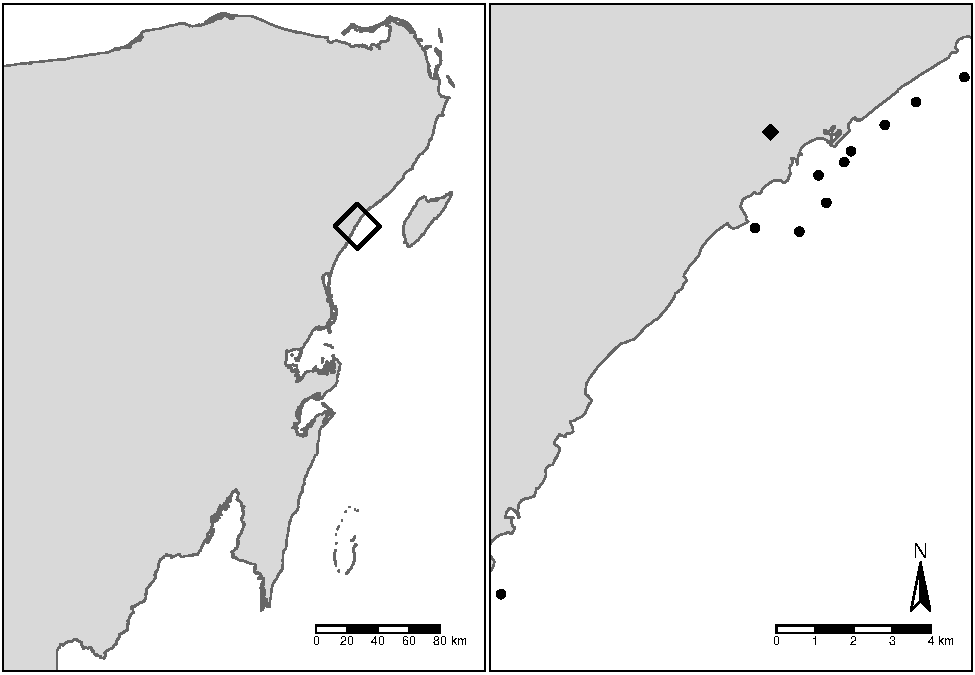
\includegraphics{Manuscript_files/figure-latex/unnamed-chunk-1-1.pdf}
\caption{\label{fig:unnamed-chunk-1}\label{fig:map}Locations where
allometric growth of lionfish (\emph{Pterois spp}) have been reported.
Sizes indicate sample size of each study, colors indicate the b
coefficient in Eq \ref{eq:allometric}}
\end{figure}

The weight at length relationship for lionfish in the central Mexican
Caribbean was calculated with the allometric growth function:

\begin{equation}
\label{eq:allometric}
TW = aTL^b
\end{equation}

Where \(TW\) is the Total Weight (gr), \(TL\) is the Total Length (mm),
\(a\) is the ponderal index and \(b\) is the scaling exponent or
allometric parameter. When \(b = 3\), it is said that the organism
exhibits a perfect isometric growth. The dependent and independent
variables were transformed via base-10 logarithms, thus the equation
becomes:

\begin{equation}
\label{eq:log-alo}
log_{10}(TW) = b\times log_{10}(TL) + log{10}(a)
\end{equation}

This can be simplified and re-written as:

\begin{equation}
\label{eq:log-alo-trans}
Y = mX + c
\end{equation}

Where \(Y = log_{10}(TW)\), \(X = log_{10}(TL)\), \(m = b\), and
\(c = log_{10}(a)\). Since \(b = m\), we will only use \(b\) throughout
the paper for simplicity. The coefficients (\(c\) and \(b\)) were
estimated with an Ordinary Least Square Regression and
heteroskedastic-robust standard error correction \citep{zeileis_2004}.
Both coefficients were tested against the null hypothesis of no change
(\emph{i.e.} \(H_0: c = 0\) and \(H_0: b = 0\)). Additionally, the
allometric parameter was tested against the null hypothesis of isometric
growth (\(H_0: b = 3\)). Coefficients were tested with a two-tailed
Student's t-test. The significance of the regression was corroborated
with an F-test.

During the review process, some studies indistinctly used \(a\) to
report either the ponderal index in \ref{eq:allometric} or the
y-intercept (\(c\)) in \ref{eq:log-alo-trans}. Others reported their
parameters as mm-to-gr conversions, but a rapid evaluation of such
parameters indicated that they were estimated as cm-to-gr conversions.
Here, all parameters are reported as TL(mm) to TW(gr) conversions. When
required, values from other studies were transformed for consistency.

Since uncertainty around estimated relationships was not reported in
some of the reviewed studies, it was not possible to test for
statistical differences between relationships. Instead, the 16
length-weight relationships were used to calculate expected weight
length observations of the organisms sampled from the Central Mexican
Caribbean (n = 109). Expected weights were divided by the observed
weights to obtain a ratio. Difference in mean weight ratios across
studies were tested with a one-way Analysis of Variance (ANOVA).

All hypothesis testing was performed with an \emph{a priori} confidence
level of \(\alpha = 0.01\) in R version 3.4.0 \citep{rcore_2017}. Raw
data and code used in this work is available at dryad.org.

\section{Results}\label{results}

The model adjusted to \ref{eq:log-alo-trans} estimated the coefficient
values at \(b = 3.2347391\) and \(c = -5.4940866\). Thus, TW (gr) can be
calculated from TL (mm) as a linear equation:
\(log_{10}(TW) = 3.2347391\times log_{10}(TL) -5.4940866\), or its
exponential form: \(TW = 3.2056297\times 10^{-6}\times TL^{3.2347391}\).
The intercept (\(c\)) and slope \((b)\) were significantly different
from zero (\(t(107) = -66.17; p<0.001\) and \(t(107) = 83.24; p<0.001\),
respectively), rejecting the null hypothesis of no change. Additionally,
the allometric factor (\(b\)) was significantly different from the value
of isometric growth of \(b = 3\) (\(t(107) = 6.04; p<0.001\)),
indicating that lionfish present allometric growth. More information on
model fit and confidence intervals for the estimated coefficients is
presented in TableS2. The relationship between Total Length and Total
Weight is presented in Figure \ref{fig:l-w-carib}.

From the 11 peer-reviewed studies including information on growth
parameters for \emph{P. volitans} and the additional calculated for the
central Mexican Caribbean, 16 parameters were identified (Table
\ref{tab:all_params}, Fig \ref{fig:all_allo}). Two studies
\citep{aguilarperera_2016,fogg_2013} reported gender-level and pooled
parameters, while the rest presented pooled results. The smallest
coefficient of determination was presented by \citet{chin_2016} with
\(R^2 = 0.8715\), while \citet{sabidoitza_2016} reported the highest
value at \(R^2 = 0.9907\). Reviewed studies presented information for
organisms obtained at depths between 0.5 and 57 m. Three studies
\citep{aguilarperera_2016,chin_2016,dahl_2014} explicitly stated that
their organisms were sampled with pole spears. Five studies
\citep{sandel_2015,barbour_2011,fogg_2013,edwards_2014,sabidoitza_2016,toledohernndez_2014}
mentioned that some of their organisms were obtained with pole spears
(or other type of harpoon), but also hand-held nets or fish traps. Two
studies \citep{deleon_2013,darling_2011} did not specify how organisms
were sampled.

Parameters from models fit to males or females exclusively tend to have
a higher steepness (\emph{i.e.} higher allometric parameter), with mean
\(\pm\) standard deviation values of \(b = 3.27 \pm 0.06\) and
\(b = 3.31 \pm 0.23\) for males and females respectively, compared to
parameters from models for pooled genders with a mean \(\pm\) standard
deviation value of \(b = 3.13 \pm 0.22\). In the case of the ponderal
index (\(a\)) and its \(log_{10}\) transformation (\(c\)), values were
higher for parameters for pooled genders. Figure \ref{fig:all_allo}
shows the weight-at-length relationships with parameters from all
studies.

There were significant differences in expected-to-observed weight ratios
estimated for each pair of parameters (F(15, 1728) = 38.26; p
\textless{} 0.001). From all allometric parameters reviewed, those of
\citet{edwards_2014} provided the lowest weight estimates, with an
expected-to-observed weight ratio of 0.98 \(\pm\) 0.23 (mean \(\pm\)
SD). On the other hand,\citet{barbour_2011} yielded the highest weight
estimates, with a mean (\(\pm\) SD) expected-to-observed weight ratio of
1.76 \(\pm\) 0.50. Predicted-to-observed weight ratios and groups
identified by Tukey's HSD (\(\alpha = 0.05\)) are presented in Figure
\ref{fig:bio_ratio}.

\clearpage

\begin{figure}
\centering
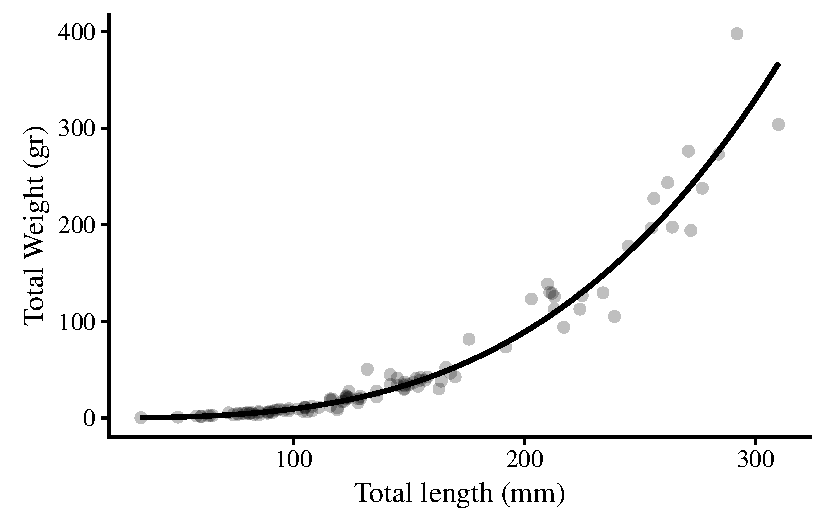
\includegraphics{Manuscript_files/figure-latex/unnamed-chunk-4-1.pdf}
\caption{\label{fig:unnamed-chunk-4}\label{fig:l-w-carib}Length-weight
relationship for 109 lionfish sampled in the Central Mexican Caribbean.
Points indicate samples, solid line indicates curve of best fit (See
Table S1).}
\end{figure}

\begin{table}

\caption{\label{tab:unnamed-chunk-5}\label{tab:all_params}Summary of 13 allometric growth parameters available for lionfish in the invaded range from peer-reviewed literature and this study. All parameters have been adjusted to convert from millimeters to grams. n = Sample size, a = scaling parameter for eq. 1, c = y-intercept for eq. 3, b = exponent or slope for eq. 1 or eq. 3, respectively. The $R^2$ column indicates reported model fit.}
\centering
\begin{tabular}[t]{lllrrll}
\toprule
Region & Sex & n & a & b & R2 & Reference\\
\midrule
Alacranes Reef, Mexico & B & 472 & 2.90e-06 & 3.30 & 0.95 & Aguilar-Perera \& Quijano-Puerto, 2016\\
Alacranes Reef, Mexico & F & 67 & 1.20e-06 & 3.47 & 0.95 & Aguilar-Perera \& Quijano-Puerto, 2016\\
Alacranes Reef, Mexico & M & 59 & 4.20e-06 & 3.23 & 0.95 & Aguilar-Perera \& Quijano-Puerto, 2016\\
Bahamas & B & - & 2.50e-06 & 3.29 & - & Darling et al., 2011\\
Bonaire & B & 1450 & 2.28e-05 & 2.89 & 0.96 & de Leon et al., 2013\\
\addlinespace
Costa Rica & B & 458 & 3.64e-05 & 2.81 & - & Sandel et al., 2015\\
Discovery Bay, Jamaica & B & 419 & 2.75e-05 & 2.85 & 0.8715 & Chin et al 2016\\
Little Cayman & B & 1887 & 3.00e-06 & 3.24 & 0.97 & Edwards et al., 2014\\
North Carolina & B & 774 & 2.89e-05 & 2.89 & - & Brbour et al 2011\\
Northern Gulf of Mexico & B & 934 & 2.10e-06 & 3.34 & 0.98 & Dahl \& Patterson, 2014\\
\addlinespace
Northern Gulf of Mexico & B & 582 & 1.40e-06 & 3.43 & 0.99 & Fogg et al., 2013\\
Northern Gulf of Mexico & M & 119 & 2.70e-06 & 3.31 & 0.97 & Fogg et al., 2013\\
Northern Gulf of Mexico & F & 115 & 6.80e-06 & 3.14 & 0.94 & Fogg et al., 2013\\
Puerto Aventuras, Mexico & B & 109 & 3.20e-06 & 3.23 & 0.9766 & This study\\
Puerto Rico & B & 227 & 8.00e-06 & 3.11 & 0.958 & Toledo-Hernández et al., 2014\\
Xcalak, Mexico & B & 2143 & 5.20e-06 & 3.18 & 0.9907 & Sabido-Itza et al., 2016\\
\bottomrule
\end{tabular}
\end{table}

\clearpage

\begin{figure}
\centering
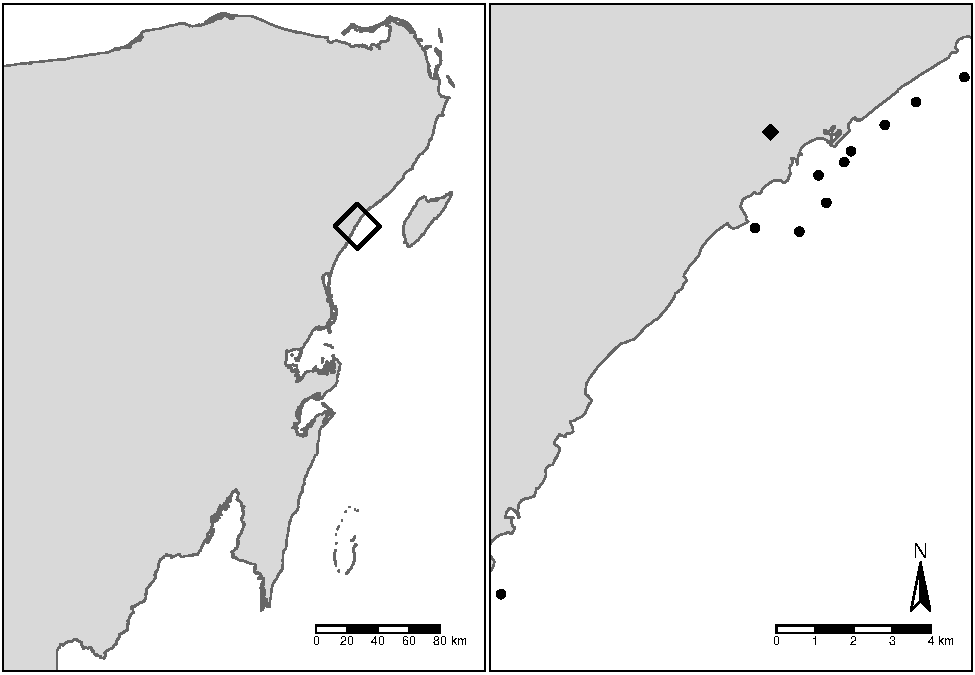
\includegraphics{Manuscript_files/figure-latex/unnamed-chunk-6-1.pdf}
\caption{\label{fig:unnamed-chunk-6}\label{fig:all_allo}Length-weight
relationships (n = 16) for eight studies, this study, and Fishbase.
Colors indicate studies from which the parameters were extracted. Solid
lines indicate that the fit was performed for males and females pooled
together. Dotted lines indicate that the regression was performed on
females, and dashed lines indicate it was performed for males.}
\end{figure}

\begin{figure}
\centering
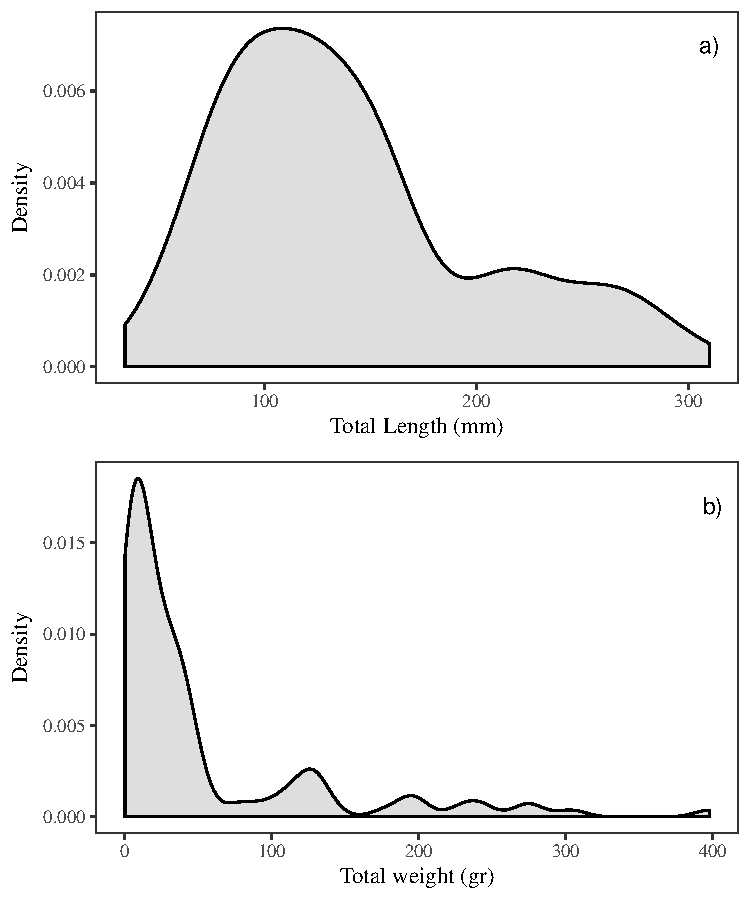
\includegraphics{Manuscript_files/figure-latex/unnamed-chunk-7-1.pdf}
\caption{\label{fig:unnamed-chunk-7}\label{fig:bio_ratio}Violin plot showing
the distribution of predicted to observed biomass ratios for 16 pairs of
allometric parameters. Red and blue circles indicate median and mean
values, respectively. Like letters indicate values that do not differ
significantly (Tukey's HSD; p \textless{} 0.05).}
\end{figure}

\clearpage

\section{Discussion}\label{discussion}

\citet{fogg_2013} uses Spine-less weight

\citet{toledohernndez_2014} compares young and wold growth

A new pair of allometric growth parameters for lionfish in the central
Mexican Caribbean are provided. This compliments existing literature for
other sites in the north (\emph{i.e.} Alacranes Reef
\citep{aguilarperera_2016}) and South (Xcalak \citep{sabidoitza_2016})
of the Mexican Caribbean. Additionally, the study identifies regional
differences in length-weight relationships. Here, we focus the
discussion on plausible causes of these differences.

The length-weight coefficients estimated in this study were within the
range identified by studies in other regions
\citep{barbour_2011,fogg_2013,aguilarperera_2016,sabidoitza_2016,edwards_2014,chin_2016,deleon_2013,sandel_2015}.
However, the ones presented here provide lower weight estimates for a
same length. Until about TL = 200 mm, there are no appreciable
differences between the parameters for organisms from the Mexican
Caribbean and those for little Cayman \citep{edwards_2014} and Jamaica
\citep{chin_2016}. Yet, for larger organisms (TL \textgreater{} 270 mm)
parameters from Costa Rica \citep{sandel_2015} and Bonaire
\citep{deleon_2013} provide similar estimates to those from this study.
Conversely, these same studies tend to estimate higher weights --as
compared to the ones reported here-- for smaller organisms, likely due
to the lack of small organisms in the samples used to estimate their
parameters.

There are evident differences in weight-at-length between organisms from
the Caribbean and Gulf of Mexico / North-Western Atlantic. Weight
estimates with parameters from the Gulf of Mexico and North-Western
Atlantic tend to be higher than those from the Caribbean. This indicates
that there are differences between lionfish across the invasion range.
Similar regional variation has been reported for age-at-length
relationships of this species \citep{fogg_2015,pusack_2016}.

Causas de las diferencias\ldots{}

These differences can have major implications in management, especially
when estimating biomass available for harvest or predicting effects on
local ecosystems, or evaluating the effectiveness of removal programs.
Using site-specific values provides a more accurate estimate of fish
biomass. Future research should try to use, to the extent possible,
parameters calculated for their region, or use different parameters to
provide upper and lower bounds in their results. At the same time, this
highlights the need for more basic research that furthers our
understanding of lionfish biology. To better manage the invasion, we
must perform research that can describe biologically important
information of lionfish throughout its invasion range
\citep{johnson_2016}.

\section{Aknowledgements}\label{aknowledgements}

I would like to thank thank Nils Van Der Haar and Michael Doodey from
Dive Aventuras as well as Guillermo Lotz-Cador who provided help to
collect samples.

\bibliography{references}

\end{document}
